\chapter{Background and Related Work}\label{chap:background}

Chapter~\ref{chap:intro} introduced the thesis problem: enabling Pepper to answer questions about its surroundings using visual perception, persistent scene memory, and language generation. This chapter reviews the background methods that directly support that goal. It does not describe the implemented architecture yet; that is the role of the following chapters. The emphasis here is on theory and related work that is later used or evaluated in the system, namely Pepper dialogue system, object detection, object persistence, grounding, scene graphs, vision-language models, Set-of-Mark prompting, and memory-based context construction.

\section{Human-Robot Interaction and Pepper Dialogue}\label{sec:hri-social-robots}

Human-robot interaction (HRI) studies how humans and robots communicate, coordinate, and evaluate each other in shared tasks. Goodrich and Schultz describe HRI as an interdisciplinary field combining robotics, human factors, psychology, design, linguistics, and computer science \cite[203--216]{goodrich_human-robot_2007}. This means Pepper is not evaluated merely as a camera or as a text generator. It is evaluated as an embodied system that speaks, displays information, is present in the scene, and sometimes fails in front of a user.

Sheridan distinguishes social interaction from supervisory control, teleoperation, and automated vehicles~\cite[525--526]{Sheridan2016HRI}. This thesis belongs to the social-interaction setting. Pepper is not used as a manipulator or navigation platform, but as a communication partner that should answer questions about its perceived environment.

Social robots are not defined only by their shape. Henschel et al.\ note that the term does not have a single universal definition, but that common elements include embodiment, autonomy, and behavior that people interpret as social~\cite[11--12]{henschel_what_2021}. This is important for Pepper: even when the robot performs a simple scripted action, users tend to interpret speech, gaze, waiting, and physical presence as parts of an interaction rather than as isolated software outputs.

Social embodiment raises expectations that a purely text-based assistant does not face. A user may reasonably expect that a robot standing in the same room can refer to objects in that room, distinguish people, or remember a previously mentioned item. Henschel et al.\ report that Pepper users expected reciprocal conversation and noticed the limits of single-turn interaction~\cite[12]{henschel_what_2021}. LLM-supported HRI has a related risk: fluent language can make users expect broader situational competence than the system actually has~\cite{kim_understanding_2024,aturhurra_leveraging_2024}.

However, embodiment can also improve how users experience a conversational system. Gava et al.\ compared an embodied robot setup with an application using the same conversational framework and report more positive ratings for the robot condition in perceived reliability, awareness of system behavior, speech quality, and ease of mistake correction~\cite{gava2024physical}. The result is preliminary, but it supports a practical design assumption used in this thesis: the robot body is not only a container for a chatbot, but part of the interaction with the human user. This makes failures of perception, latency, and memory visible to the user, but it also makes grounded answers more useful when they work.

Pepper already provides useful interaction services through NAOqi, including speech, tablet output, camera access, people perception, behavior control, and dialogue modules~\cite{softbank_python_sdk_2026}. These services make Pepper a practical platform for situated dialogue, because the same application can listen, speak, move, display information, and capture images. However, the native stack does not by itself provide open-ended grounded answers about changing visual memory~\cite{softbank_alspeechrecognition_2026}.

Pepper dialogue is commonly built with ALDialog and QiChat-style topics. A topic defines patterns that can match recognized utterances and proposals that the robot can say. This is a rule-based dialogue management approach: it is reliable for bounded commands, confirmations, and menu-like interaction, but it does not infer arbitrary facts about the world. Its strength is that recognized language can be routed to deterministic actions, including Python-side methods that make the robot speak, move, show tablet content, or call external services, with close to no latency~\cite{noauthor_qichat_nodate}.

Dynamic concepts make this rule-based layer more flexible. Instead of hard-coding every possible object name or relation into the grammar, the application can update a concept at runtime with scene-dependent words~\cite{noauthor_qichat_nodate}. In a scene-aware dialogue system, such concepts can contain currently visible object labels, attributes, relations, or pregenerated questions. This allows a relatively static QiChat topic to stay connected to changing visual memory: the grammar recognizes the user's intent, while external perception and memory provide the current content.

\section{Object Detection and Object Persistence}\label{sec:object-detection-tracking-reid}

Object detection provides the first layer of visual evidence. It is the task of identifying object instances in an image and localizing them, most commonly by bounding boxes. A detector maps an image \(I\) to a finite set
\[
\mathcal{D}(I)=\{(b_i,\ell_i,s_i)\}_{i=1}^{N},
\]
where \(b_i\) is a bounding box, \(\ell_i\) is a class label, and \(s_i\) is a confidence score~\cite[Section 50.4.1]{foundationsCVbook}. %In this thesis, detections are not final answers. They are object hypotheses from which identity persistence, attributes, relations, memory updates, and dialogue context are later constructed.

Modern object detection was strongly shaped by convolutional neural networks, which exploit spatial structure in images through learned local filters and hierarchical visual features~\cite[439]{lecun_deep_2015}. A major practical line of work is represented by YOLO, short for \emph{You Only Look Once}. YOLO-style detectors process the image in a single forward pass and predict bounding boxes, confidence scores, and class probabilities from dense image features~\cite{redmon_you_2016}. This makes them attractive when latency matters. Modern YOLO implementations still follow this general idea while using improved backbones, multi-scale feature fusion, detection heads, confidence filtering, and usually non-maximum suppression to remove redundant boxes~\cite{sapkota_ultralytics_2026}.

DETR-style detectors take a different view. Instead of treating detection primarily as dense prediction over spatial feature locations, DETR formulates detection as set prediction~\cite{carion_end--end_2020}. Learned object queries predict a set of object hypotheses, and training matches predictions to ground-truth objects with bipartite matching. The result is conceptually different from YOLO-style dense detection: YOLO emphasizes efficient single-pass dense prediction, while DETR emphasizes direct set prediction and reduces dependence on heuristic duplicate removal. This family is relevant to the thesis because the implemented system uses RF-DETR as one detector backend. RF-DETR follows the real-time detection-transformer direction and is designed around accuracy-latency tradeoffs for practical detection~\cite{robinson_rf-detr_2026}. The important background point is not the full architecture of RF-DETR, but the role of a detector backend: it supplies localized object instances that the rest of the scene-aware dialogue pipeline can use.

Closed-vocabulary detectors predict labels from a fixed ontology. COCO is a common example of such an ontology, containing everyday object categories widely used in detection benchmarks and pretrained detectors~\cite{lin2015microsoftcococommonobjects}. Closed-vocabulary detection is practical and stable, but it is also limited by the labels available during training. In an office, classroom, or computer laboratory, users may refer to objects that are too specific, rare, or task-dependent for the detector's fixed label set.

Open-vocabulary detection addresses this limitation. Models such as OWL-ViT and OWLv2 compare visual regions with text queries, allowing labels to be supplied at inference time~\cite{minderer_simple_2022,minderer_scaling_2024}. This is attractive for dialogue because users may ask about ordinary environment-specific objects. The cost is that the detector becomes sensitive to prompt wording, label granularity, and score calibration. Therefore, open-vocabulary detections must be treated as evidence rather than as guaranteed facts.

Object detection is inherently frame-local. It does not decide whether a chair seen now is the same physical chair seen earlier. In continuous video streams, this is usually addressed by multi-object tracking. Tracking-by-detection methods such as SORT, Deep SORT, and ByteTrack associate detections across adjacent frames using motion, geometry, confidence, and sometimes appearance information~\cite{bewley_simple_2016,wojke_simple_2017,zhang_bytetrack_2022}. These methods are effective when consecutive frames are temporally and spatially close.

Pepper's observations in our implementation violate this assumption. The robot may capture one image, speak, move its head, capture another image from a different viewpoint, and later answer a follow-up question. Between such observations, an object may shift strongly in image coordinates or disappear from the field of view. Pure frame-to-frame tracking is therefore not sufficient for persistent scene memory.

This motivates re-identification (Re-ID). Re-ID asks whether two observations correspond to the same physical instance across different times, views, or contexts~\cite[22--23]{zheng_object_2024}. For the present thesis, the important idea is appearance-based matching of object crops. A crop from the current image can be compared with crops stored in gallery; if the visual evidence is sufficiently similar and the labels are compatible, the system may treat the detections as the same object instance.

Re-ID is often described as a query-gallery problem. The current crop is the query, and previously stored crops form the gallery. A feature extractor maps crops into an embedding space where instance-specific cues are preserved. At the same time, the embeddings must be robust to noise, such as change in lighting, scale or viewpoint~\cite[22]{zheng_object_2024}. This task is thus very different from ordinary classification solved by object detection: the goal is not only to say that two crops are both chairs, but to decide whether they are the same chair.

Pepper also provides native people-perception modules through NAOqi API. ALPeoplePerception can expose visible people and their associated IDs. These can in turn be used to fetch related signals, e.g., estimated age, distance from robot, gaze direction. In addition, ALFaceDetection can detect and optionally recognize faces after learning.\footnote{See the Aldebaran documentation for ALPeoplePerception and ALFaceDetection: \url{http://doc.aldebaran.com/2-4/naoqi/peopleperception/alpeopleperception.html} and \url{http://doc.aldebaran.com/2-4/naoqi/peopleperception/alfacedetection.html}.} These modules are useful for human-centered interaction, but they are not a general object-persistence solution. They apply primarily to people and depend on visibility, pose, distance, and prior enrollment. In the thesis system, they are best understood as auxiliary robot metadata that can support visual memory.


\section{Grounding and Scene Graph Generation}\label{sec:grounding-sgg}


In robotics, grounding means linking linguistic expressions to entities, attributes, and relations in the perceived world. Lemaignan et al.\ describe situated grounding as a connection between perception, symbolic knowledge representation, and dialogue processing~\cite[181--182]{lemaignan_grounding_2012}. For the present thesis, the important point is that grounding is not achieved by adding an image to a prompt alone. The system needs a representation in which a phrase such as \enquote{the object next to the laptop} can be connected to perceived objects and relations.

A list of detections is insufficient for many grounded questions. It may contain object labels and bounding boxes, but on its own it does not say whether a cup is on a table, whether a person is wearing glasses, or whether a keyboard is to the left of a monitor. 

At first, captions seem to provide a sufficient description of a scene in natural language, which could be used by a conversational robot systems as grounding evidence~\cite{grassi_grounding_2024}. However, there is a more effective concept fit for this task.  

Scene graphs provide a compact representation for this missing structure. Johnson et al.\ define a scene graph as a data structure that encodes object instances, object attributes, and relationships between objects~\cite[3668--3669]{johnson_image_2015}. A simple formulation is
\[
\mathcal{G}=(\mathcal{O},\mathcal{E}),
\]
where \(\mathcal{O}\) is a set of object instances and \(\mathcal{E}\subseteq \mathcal{O}\times\mathcal{R}\times\mathcal{O}\) is a set of directed relationship edges. A binary relation can be written as a subject-predicate-object triplet \((s,p,o)\), for example \((\text{cup},\text{on},\text{table})\). Attributes can be stored as node properties or unary labels. Zhu et al.\ summarize scene graphs in the same practical way: as structured representations of objects, attributes, and relationships~\cite[3]{zhu_scene_2022}.

Scene Graph Generation (SGG) is the task of producing this structure from visual input. Classical SGG is often organized in two stages: first detect objects, then predict predicates for candidate object pairs. Learned methods rely on object labels, visual features, pair geometry, context, and dataset priors to predict relation triplets correctly~\cite[5]{zhu_scene_2022}. 

MAYBE REMOVE: The difficulty of SGG also lies in relationship prediction. Predicate distributions are long-tailed, relation labels can be semantically ambiguous, and object-detection errors propagate into the graph. A missed object removes all relations involving that object. A wrong label or an unstable identity can make a correct relation unusable in dialogue.


RelTR is a representative of the one-stage alternative. It builds on the set-prediction idea from DETR, but predicts a sparse set of subject-predicate-object triplets directly instead of enumerating all possible object pairs and classifying predicates for each pair. At a high level, RelTR uses entity representations, subject and object branches, and learned triplet queries to decode relation candidates. The final output includes subject and object classes and boxes together with a predicate label ~\cite{cong_reltr_2023}. 


A newer option is VLM-based SGG. Instead of treating relation prediction only as a fixed predicate-classification problem over detected object pairs, recent work formulates SGG as a promptable image-to-text or image-to-sequence generation problem. This is attractive when the target vocabulary is open, domain-specific, or not well covered by standard SGG datasets. 

IndVisSGG is a relevant example. It uses VLMs for scene graph generation in industrial spatial-intelligence settings. The method is built around GPT-4V-based multi-agent processing over video frames. Its inputs include visual information, predefined object categories, predicate dictionaries, and positive and negative examples. The prompt is structured into scene-graph information, triplet extraction criteria, and output-format requirements. The process first extracts spatial-temporal triplets from vision information, then uses multiple expert agents to check for omissions, redundant entities, and predicate-rule violations, and finally summarizes spatial and interactive relations into the final graph. Figure~\ref{fig:indvissgg-background} illustrates this pipeline~\cite{wang_indvissgg_2025}.

\begin{figure}[!htbp]
\centering
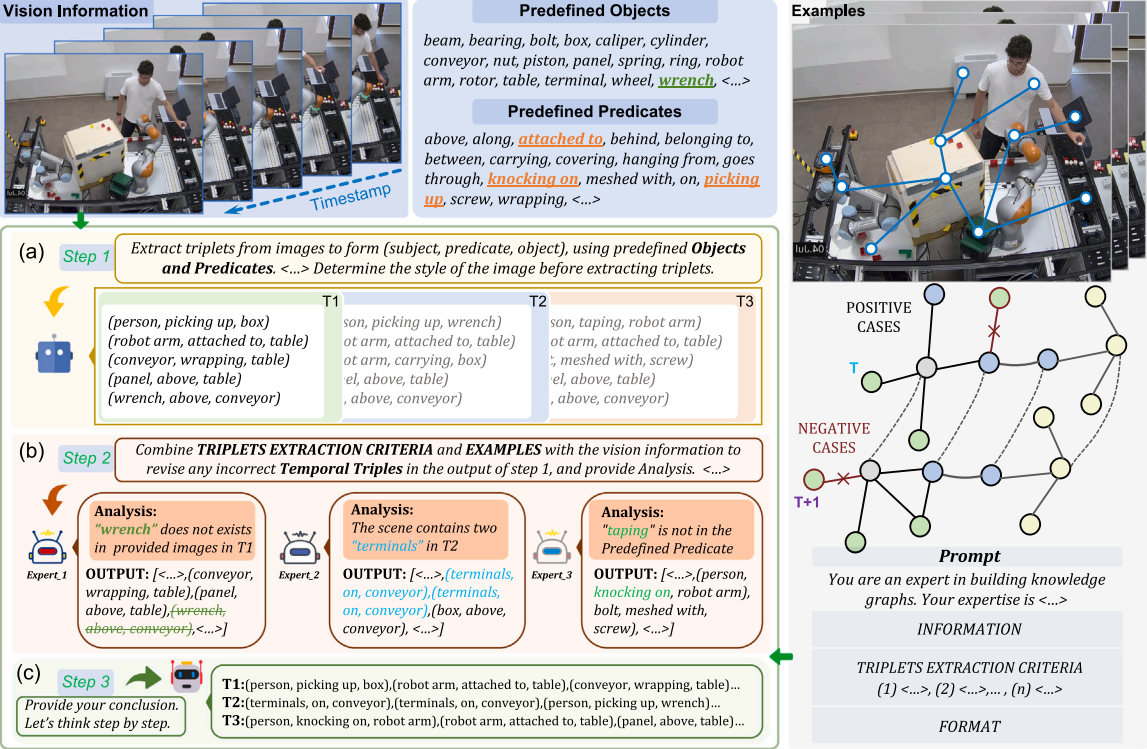
\includegraphics[width=0.95\linewidth]{pics/indvissgg_screenshot.png}
\caption{Architecture of IndVisSGG. The method combines visual information, predefined objects and predicates, examples, triplet extraction criteria, and a multi-agent GPT-4V process for extracting, checking, and summarizing scene-graph triplets. Reproduced from Wang et al.~\cite{wang_indvissgg_2025}.}
\label{fig:indvissgg-background}
\end{figure}

IndVisSGG is close to the methodological direction of this thesis even though the domain is different. It uses a constrained object and predicate vocabulary, prompt criteria, visual input, and correction around generated triplets. 

PGSG, or Pixels to Scene Graph Generation with Generative VLMs, provides another example of this direction. Li et al.\ formulate open-vocabulary SGG as generation of a textual scene-graph sequence from an image. Their method uses scene-graph prompts with relation-aware tokens to represent subject-predicate-object structure, followed by a relation-construction module that converts the generated sequence into instance-level triplets~\cite{li_pixels_2024}. 

PGSG also includes grounding and category conversion modules to recover bounding boxes and map generated words to benchmark object and predicate categories. This is important for open-vocabulary SGG because predicates can be generated from the VLM's language space rather than selected only from a closed classifier head~\cite{li_pixels_2024}. 

For this thesis, the relevance is mainly methodological: it supports the use of VLMs as flexible relation generators for a domain-specific vocabulary, while also showing why generated graphs still require grounding, normalization, filtering, and schema control before they can be stored in scene memory.

The limitation is output control. A generative model may invent unsupported relations, use inconsistent predicate names, ignore object identifiers, or produce malformed structure. Therefore, VLM-based SGG normally needs validation, normalization, and evaluation against a task-specific vocabulary.

A further practical issue is reference alignment. If a VLM is asked to produce relations between detected objects, it must refer to the same object instances as the detector and the memory system. This motivates Set-of-Mark prompting, discussed next.

\section{Set-of-Mark Prompting}\label{sec:set-of-mark}

Set-of-Mark prompting marks visible image regions with explicit identifiers before the image is passed to a VLM. Instead of asking the model to infer which of several similar chairs is meant by \enquote{the chair}, the prompt can ask about \enquote{object 4}. Yang et al.\ describe this as a visual prompting method: the original image is transformed into a marked image, and the VLM is queried using the marked image rather than the unmodified one. Their central observation is that marks such as numbers and masks make image regions both visually highlighted and linguistically referable, which in turn produces more factually correct results~\cite{yang_set-of-mark_2023}. The technique is illustrated in Figure~\ref{fig:som-prompting-background}

\begin{figure}[!htbp]
\centering
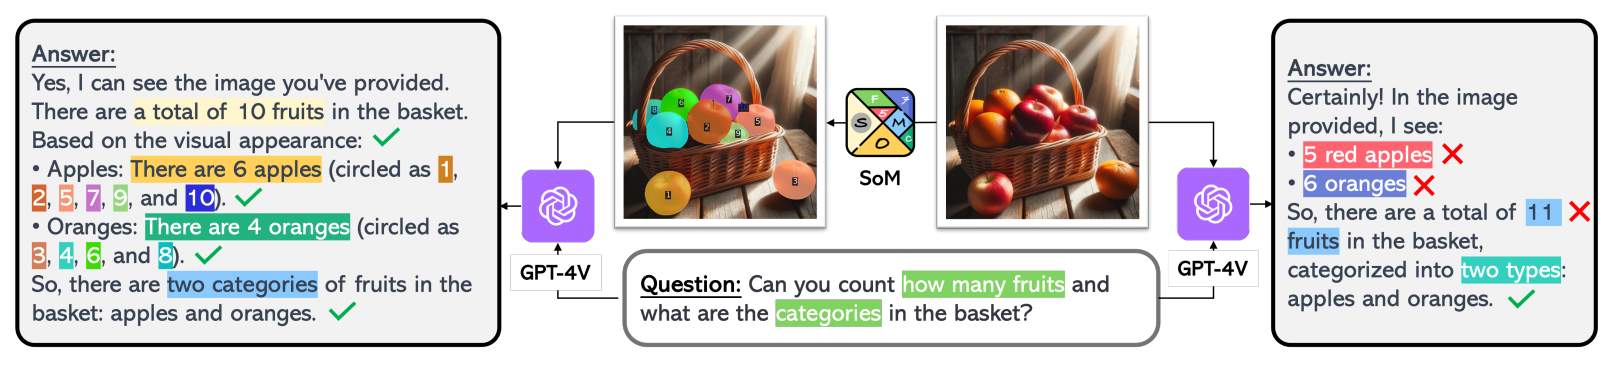
\includegraphics[width=1\linewidth]{pics/som_prompting_original_pic.png}
\caption{Illustration of standard VLM prompting compared with Set-of-Mark prompting. The visual marks make image regions explicitly referable in the text prompt, reducing ambiguity when the model must answer about a specific object, increasing the probability of correct answer. Reproduced from Yang et al.~\cite{yang_set-of-mark_2023}.}\label{fig:som-prompting-background}
\end{figure}

The method has two main components. First, the image is partitioned into meaningful regions, for example with segmentation or detection models. Second, each region is overlaid with a unique mark, usually a number, letter, mask, box, or a combination of these. The mark must be easy for the VLM to perceive and easy for the language model to mention in text. This is why numeric or alphabetic labels are useful: the model can answer with \enquote{region 3} or \enquote{object B} instead of producing uncertain coordinates. However, in low-resolution or cluttered images, the marks can cover visual evidence or add noise which might hinder the overall performance.

For scene-aware dialogue, the main value of Set-of-Mark prompting is alignment. Detector IDs, graph nodes, VLM references, tablet visualization, and later spoken answers can all refer to the same marked object. This is particularly important in scenes with repeated objects, such as multiple chairs, monitors, books, or people.

\section{Language Models, Vision-Language Models, and Scene Context}\label{sec:llms-vlms-context}

Large language models are useful in dialogue because they can generate fluent responses conditioned on an instruction and context. Instruction tuning and preference-based alignment make such models more suitable for interactive use than raw pretrained language models~\cite{ouyang2022traininglanguagemodelsfollow}. For grounded robot dialogue, however, fluency is not enough. The model can only answer correctly about the scene if the relevant scene evidence is present in its context or accessible through a retrieval mechanism.

Vision-language models extend language generation or visual representation learning with image input~\cite[2--3]{zhou_large_2026}. Some models use shared image-text embedding spaces, which are useful for retrieval and open-vocabulary perception. Others connect visual encoders to language models and generate text conditioned on both the prompt and the image. This makes VLMs attractive for captioning and for producing draft scene graphs. The same property also creates risk: a VLM may hallucinate objects, ignore a required schema, or use relations outside the intended vocabulary.

In a social robot, such mistakes are not merely technical. The user may see the same room as the robot, so an unsupported answer can immediately break trust or fail to fulfill the user's information need. For this reason, grounded systems should treat LLM and VLM outputs as mere hypotheses to be constrained, checked, or stored with provenance rather than as direct truth.

One way to lower the hallucination risk is to provide the model with a relevant context. Retrieval-Augmented Generation (RAG) combines a generator with external evidence retrieval~\cite{lewis_retrieval-augmented_2020}. In ordinary text settings, the external evidence is often a set of document chunks which are retrieved based on their semantic similarity with the query. 

For scene-aware dialogue, the relevant context is a scene memory which is more naturally graph-like: objects are nodes, attributes are node properties, and relationships are edges. A question such as \enquote{what is next to the monitor?} should retrieve the monitor and its graph neighborhood, not merely the most semantically similar text fragment.

Cache-Augmented Generation (CAG) uses a different assumption: if the relevant knowledge is bounded and fits into the model context or cache, it can be loaded once and reused without online retrieval~\cite{Chan_2025}. This idea is relevant for small current-scene memories, where the full scene summary may fit into a prompt. Its limitation is the same as in any context-construction method: irrelevant or stale context can distract the model, while missing context prevents grounded answers.

The background consequence for this thesis is pragmatic. Captions, scene graphs, cached questions, and object-focused summaries are different ways of moving visual memory into language-model context. The implementation details belong to later chapters, but the common principle is simple: the dialogue model should answer from a maintained scene state, not from its pretrained world knowledge alone.

\section{Pepper Robot Specification}\label{sec:pepper-specification}

Pepper is a humanoid social robot designed by Aldebaran Robotics in 2014 and manufactured until 2020. It provides speech output, microphones, cameras, a chest tablet, expressive head and arm motion, and a mobile base. In this thesis, Pepper is treated primarily as an embodied communication platform rather than as a manipulation platform. Its role is to support situated dialogue about the visible environment, not to physically modify that environment.

Pepper's technical specification is relevant because it defines the computational and software constraints under which the system must operate. Public specifications list an Intel Atom E3845 CPU, 4 GB RAM, and 32 GB eMMC flash memory in the main CPU module, together with RGB cameras, microphones, speakers, sonars, lasers, bumpers, and the chest tablet.\footnote{See the Pepper technical specifications: \url{https://aldebaran.com/support/kb/pepper/general/pepper-technical-specifications/}.} These resources are appropriate for Pepper's native interaction, sensing, motion, and dialogue modules, but they provide limited headroom for computationally demanding neural inference. 

In addition, Pepper's NAOqi software environment relies on legacy Python 2 interfaces, while contemporary ob\-ject-de\-tec\-tion, vi\-sion-lan\-guage, lan\-guage-mod\-el, and scene-graph-gen\-er\-a\-tion frameworks are developed primarily for modern Python 3 ecosystems and often assume hardware acceleration. For this reason, these models are not deployed directly on the robot. Instead, Pepper is used as the embodied interaction client, while the more demanding perception and lan\-guage-pro\-cess\-ing components are executed on an external machine. This constraint motivates the cli\-ent-serv\-er architecture described later in the thesis.

%The tablet is also part of the interaction setting, not merely a display peripheral. It can show visual state, possible questions, memory content, or disambiguating information~\cite{softbank_peppers_tablet_2026}. In grounded dialogue, this matters because it gives the user a way to inspect what the robot believes it has seen. The tablet can therefore reduce the mismatch between the user's view of the scene and the robot's internal scene memory.

This chapter therefore narrows the background to the methods directly needed later. Pepper dialogue provides the interaction interface, Pepper hardware defines the computational and software constraints, object detection and persistence provide visual entities, scene graphs provide structured memory, Set-of-Mark prompting helps align VLM references with detected objects, and language models turn selected scene context into spoken answers.